



\chapter {Contribution 1 BALANCE}
\section{Introduction}
Globally, 34\% of adults were overweight or obese in 2008 \cite{kimokoti_diet_2011}. While this has been a concern particularly in Westernized countries, the epidemic is spreading globally: Nauru in the Oceania reported the greatest gain in BMI globally \cite{finucane_national_2011}. Overweight and obesity are major risk factors for cardiovascular disease (CVD), Type 2 diabetes mellitus, and certain forms of cancer \cite{guh_incidence_2009} \cite{calle_overweight_2004}. 

Self-monitoring, defined as the process of observing and recording target behavior, has been identified as a key component of behavior change in general \cite{kanfer_self-monitoring:_1970} and for weight loss in particular \cite{michie_effective_2009} \cite{burke_effect_2011}. Of the people who have lost weight and kept it off (as registered with the Weight Loss Registry), the key behavior that correlates highly with losing and keeping weight off is the practice of self-monitoring both food (energy) intake and physical activity (energy expenditure) [ref]. In general, people tend to underestimate their energy intake, while overestimating how many calories they burn in physical activity (energy expenditure) [ref]. This tendency results in an unawareness of the actual overall balance of caloric intake and expenditure, which results in weight gain. 

People underestimate energy intake for a variety of reasons, including a lack of awareness of how many calories are in food [ref]; what an appropriate serving size is [ref]; erroneous estimates of how much of a food has been eaten [ref]; and neglecting to consider calorie dense condiments or additions to a food [ref]. This effect is magnified when a person does not document what they eat as soon as they eat it, and time passes between consumption and recording [ref]. Additionally, although reflecting on food intake in the past (e.g., earlier in the day) may help raise an individual's awareness of calories in given foods, it does not enable them to make good decisions in the moment. Timely access to calorie data could help people not only capture and understand how many calories they have already consumed for the day, but also make better decisions going forward. 

People also underestimate the number of calories they burn over time. An estimate of energy expenditure by a person in a given time period is the sum of three items: the base metabolism for that individual (how many calories their body consumes for basic bodily function), the amount and intensity of intentional exercise (e.g., going for a run) and the amount and intensity of unintentional exercise (e.g., how much walking versus sitting a person does). It is relatively easy for people to measure their intentional exercise, as it's usually well-defined. However, humans tend to vastly underestimate their unintentional exercise [ref]. Readily available technology such as wearable sensors can keep track of general activity for an individual, allowing them to more closely track energy expenditure over time. 

The BALANCE project was a multi-year, interdisciplinary project with the goal of designing, building, and evaluating a mobile-phone based application to help people overcome these challenges of tracking their overall balance of energy intake and expenditure. It combines a wearable device that calculates caloric expenditure with a mobile phone that runs software that includes a food diary to track caloric intake. The software also includes a visualization that reports the real-time energy balance for the day. The wearable device is built using the multi-sensor board (MSB) [ref]. The MSB contains an accelerometer, now standard in mobile phones, as well as other sensors that aide in physical activity detection.  

The software consisted of three main components: a ``fuel gauge'' visualization that reflects the current caloric balance; a food diary; and a physical activity diary. The food diary requires users to enter the details of what they eat, while the physical activity diary accepts input from the external MSB device that calculates most calories burned from physical activity (the exception being water or high-impact sports, which need to be manually entered).
 
\subsection{Project Overview}
This project consisted of many phases and many people were involved. We started with brainstorming designs for and evaluation of the fuel-gauge visualization; executed a paper prototype evaluation of the software based on specified need, goals and reviews of similar tools; built an initial prototype on a feature phone platform; validated the algorithms on the MSB for calculating calorie expenditure; and executed an iterative design and implementation process of the application on a smartphone. Finally, the smartphone software and MSB were combined and validated overall. My primary contribution to this project was the design and implementation of the smartphone software. The rest of this chapter describes the process and final product in further detail. 

Multiple documents describe contributions to the BALANCE project. Tamara Denning contributed to the initial design and paper prototype evaluations [ref]. Deonna Hughes designed, conducted, and analyzed the focus groups and prototype iterations [ref, ref]. She looked at two metrics for improvement from iteration to iteration. The first was the result of standardized usability questionnaires (CSUQ [ref] and MPUQ [ref]); the other was the time between when participants ate a food and when they entered it in the diary. Neither metric showed significant improvement in the prototype over 5 iterations. I discuss this in further detail later in this chapter. Jonathan Lester designed and evaluated the calorie expenditure algorithms [ref, ref], employing a gold-standard oxygen-consumption evaluation methodology. Algorithms using the MSB sensor data were 89.54\% (+/- 7.25\%) accurate in the lab and 79.8\% (+/- 9.48\%) in the field.  Heather Snively designed and conducted the overall system validation [ref, ref]. Participants used the entire system for 4 days, tracking their food intake on days 1, 3, and 4. On day 2 participants provided a 24-hr recall of what they ate on day 1, which was compared to entries in the food diary on the first day. The average percent calorie difference between the mobile phone food diary and the 24-hr recall was 9 +/- 18\% [ref].  

\section{Fuel-Gauge Visualization}
The goal of the BALANCE project was to combine a food diary to collect information about energy intake, a physical activity component (diary + MSB) to collect energy expenditure information, and the fuel gauge visualization to show the current energy balance throughout the day. The heart of the system was a unifying user interface on a mobile phone. 

The first investigation focused on the fuel-gauge visualization. It was important that the visualization provide the current overall energy balance, but it was unclear what other information would be necessary or relevant. Additionally, it was important to produce a visualization that was understandable at a glance, provided more meaning upon reflection, and worked within the constraints of the target device in terms of size and resolution. One concern was the level of abstraction: whether the visualization depicts a concrete, physical world phenomena or a more mathematically-oriented graph view. In this section, I describe a user study to collect feedback on a wide range of potential visualizations. 

\subsection{Participants}
12 participants (10 female and 2 male) were recruited from a university community. Ages ranged from 18-50, with a majority (8) in the 30-40 year age range. 

\subsection{Procedure}
Participants were asked to come to the lab, where they filled out a survey collecting basic demographic information. Next, the interviewer conducted a survey where participants were asked to rate the desirability of given features for food and exercise applications on a mobile phone and to talk about what they had already eaten that day (or the previous day, depending on time of interview), including context (what they ate, how much, where, when, and how much that meal varies for them). 

Next, participants were shown the different visualizations. Each visualization depicted the same four situations: the start of the day, before any food is entered or calories expended; the end of the day, when more than the day's goal had been consumed and expended; and two points in between, showing various balance levels. 

There were two categories: graphs (two total) and visualizations (five total). Participants were asked to rank their preferred visualizations within each category and offer comments. 

\subsection{Instruments}
The team brainstormed seven candidate visualizations. Ideas ranged from abstract charts to concrete metaphors. Previous work investigates the value of having abstract versus concrete representations [ref], so we aimed for a wide range at this point in the design process. 

The main goal of the visualization is to depict the current energy intake/expenditure balance. Other pieces of information that could be helpful included: 
\begin{enumerate}
\item what the goal calorie expenditure and intake is for a current day;
\item progress toward that goal/target over the course of the day; and
\item whether or how much the user was over the intake or expenditure goal for the day. 
\end{enumerate}

Mobile phone displays vary greatly in their capabilities, specifically in size and resolution. To present the visualizations in the context that they would appear to users, the visualizations were generated on the mobile phone device, saved as screenshots, then printed on paper. It was important that the visualizations reflect the constraints of the display, as well as the fact that these were early sketches. Presenting the visualizations on the actual mobile device could raise user
 expectations of the visualization, while paper prototypes and screenshots help to restrain user expectations appropriately. The visualizations were deliberately ``rough'' and unrefined, to target the level of refinement ideal for a paper prototype. 

\begin{figure}[ t ]
\begin{center}
\subfloat[ Viz1 ]{
\setlength\fboxsep{0pt}
\setlength\fboxrule{0.5pt}
\fbox{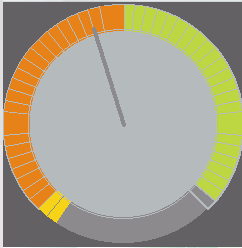
\includegraphics[ width =2.5cm ]{./images/cont1/Viz_1_10}}
\label{fig:viz1}
}
\subfloat[ Viz2 ]{
\setlength\fboxsep{0pt}
\setlength\fboxrule{0.5pt}
\fbox{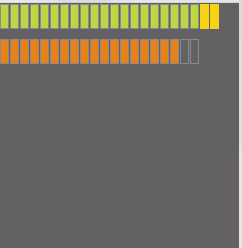
\includegraphics[ width =2.5cm ]{./images/cont1/Viz_2_5}}
\label{fig:viz2}
}
\subfloat[ Viz3 ]{
\setlength\fboxsep{0pt}
\setlength\fboxrule{0.5pt}
\fbox{
\includegraphics[ width  =2.5cm ]{./images/cont1/Viz_3_3}}
\label{fig:viz3}
}
\subfloat [ Viz4 ]{
\setlength\fboxsep{0pt}
\setlength\fboxrule{0.5pt}
\fbox{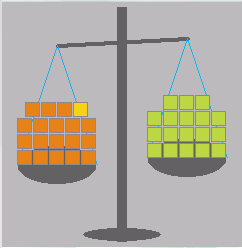
\includegraphics [ width  =2.5cm ]{./images/cont1/Viz_4_4}}
\label{fig:viz4}
}
\subfloat [ Viz5 ]{
\setlength\fboxsep{0pt}
\setlength\fboxrule{0.5pt}
\fbox{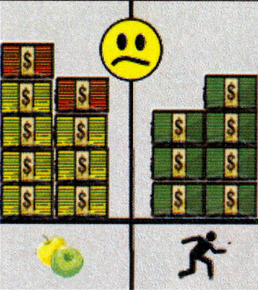
\includegraphics [ width  =2.5cm ]{./images/cont1/money}}
\label{fig:viz5}
}
\subfloat [ Graph1 ]{
\setlength\fboxsep{0pt}
\setlength\fboxrule{0.5pt}
\fbox{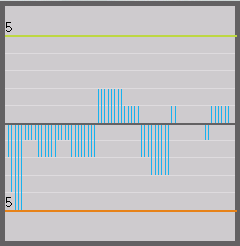
\includegraphics [ width  =2.5cm ]{./images/cont1/Viz_6_1}}
\label{fig:graph1}
}
\subfloat [ Graph2 ]{
\setlength\fboxsep{0pt}
\setlength\fboxrule{0.5pt}
\fbox{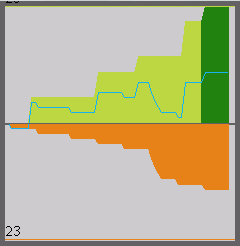
\includegraphics [ width  =2.5cm ]{./images/cont1/Viz_8_4}}
\label{fig:graph2}
}
\caption{A bunch of screens. Look at subfig and continueFloat to help wrap some of the images to the next line.}
\end{center}
\end{figure}


\subsection{Results and Discussion}
We rated visualizations based on the number of \#1 rankings it received.  
In the graph section, we saw that participants strongly preferred Graph 2, giving it 10 \#1 rankings. However, feedback overall was that the graphs were challenging to understand at a glance, and needed more explanation. 
In the visualization section, 5 participants ranked Viz1 \#1, making it clearly preferred. Participants liked the ``meter'', and the comparison it provided (P2). It was also remarked to be ``clear, straightforward'', that it ``seems useful'' and ``shows a good balance [of detail]'' (P5).  Viz 3 received all \#4 and \#5 rankings, because it ``doesn't show progress and amounts'' (P12), and is ``more confusing'' (P7) . Viz 5 received a wider range of rankings, the feedback on it was strong (it's ``a little too judgmental'', and ``not neutral enough'' [P3];P5: ``means nothing with respect to food, smileys are annoying''; P2: ``faces are more discouraging than encouraging-critique''). 
 
Feedback from the user population indicated that Viz1 is the preferred visualization. Participants liked that it showed the current energy balance while also showing progress towards daily goals or targets, for both energy intake and expenditure. Feedback indicates that the most simple feedback shown (direction and magnitude of energy imbalance, Viz3) does not show enough information and is unsatisfying. Participants in general found the time-based visualizations too complicated to quickly understand, and didn't believe that the balance over time was useful information. 

Feedback also indicated that participants felt the physical metaphors such as the scales depicted in Viz4 and Viz5 were symbols that were too rich and the imagery too loaded for simple feedback. The scale metaphor reminded users that if their energy balance was off, their own scale would be tipping. 
 Users were vocal against the use of money to represent caloric intake and expenditure. While the money ``earned versus spent'' metaphor could be powerful to communicate the ``calories in equals calories out'' concept, people reported that both money and weight were too emotionally charged and they didn't want to put the two together. The smiley faces in Viz5, while encouraging when the user is doing well, can be discouraging when the user is struggling. Indeed, this is consistent with [ref], which explores communicating positive and negative affect in feedback mechanisms. 

\section{Prototype, V1 (Feature Phone \& USDA Food Database)}
The next phase of the BALANCE project was the design and development of the first mobile phone prototype. The design of this prototype was informed by a review of existing related products (to identify key desired features), a paper prototype process, and the visualization feedback process described above. 
This prototype was built on the Symbian S60 feature phone platform (a top-of-the-line mobile phone platform at the time). Characteristics of mobile phones running the Symbian S60 platform included a relatively powerful processor and ample storage, the ability to develop and run custom software, and high quality cameras, but had a small display and 12-key keypads. 
This prototype was built with the commonly used, freely available USDA food database (SR21) [ref]. The database schema is in [ref]. Additionally, we added an index based on the FOOD\_DES.FoodName column.  User search requests were turned into a wildcard LIKE query against the index. Multiple words in the user request were split ANDed together. 





\begin{figure}[ t ]
\begin{center}
\subfloat[  ]{
\setlength\fboxsep{0pt}
\setlength\fboxrule{0.5pt}
\fbox{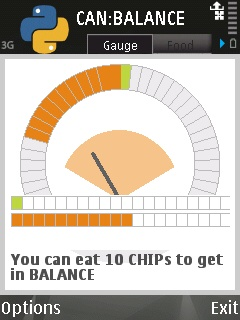
\includegraphics[ width =2.5cm ]{./images/cont1/fig3a}}
\label{fig:fig3a}
}
\subfloat[  ]{
\setlength\fboxsep{0pt}
\setlength\fboxrule{0.5pt}
\fbox{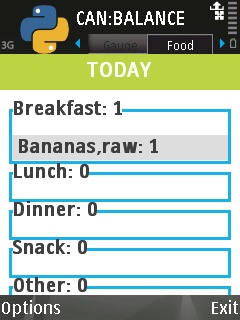
\includegraphics[ width  =2.5cm ]{./images/cont1/fig3b}}
\label{fig:fig3b}
}
\subfloat [  ]{
\setlength\fboxsep{0pt}
\setlength\fboxrule{0.5pt}
\fbox{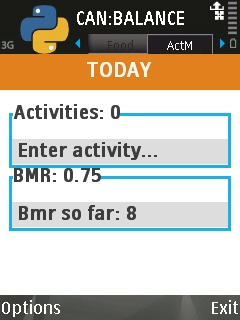
\includegraphics [ width  =2.5cm ]{./images/cont1/fig3c}}
\label{fig:fig3c}
}
\subfloat [  ]{
\setlength\fboxsep{0pt}
\setlength\fboxrule{0.5pt}
\fbox{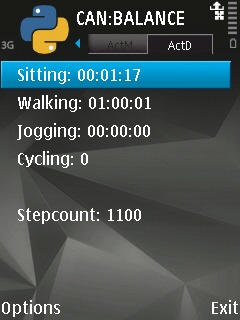
\includegraphics [ width  =2.5cm ]{./images/cont1/fig3d}}
\label{fig:fig3d}
}
\caption{Nokia prototype main screens}
\end{center}
\end{figure}

\subsection{Description}
The BALANCE software consisted of four main screens (Figure 3): The overall balance visualization (a), the food diary that shows which foods have been entered today (b), and two activity screens. The first activity screen (c) shows intentional activity that is not detected by the MSB (for example, water sports such as swimming) and is therefore entered by the user, and energy expenditure due to base metabolic rate (BMR-the calories a body uses for basic metabolic processes like breathing). The second activity screen (d) shows activity detected by the MSB unit, and its contribution to overall energy expenditure. 
We adopted an overall simplifying construct for calorie counting called ``CHIPs'': [acronym here][ref]. A CHIP is simply a unit of 100 calories. Humans find it easier to count and keep track of larger increments (smaller numbers), so in the BALANCE software, all calorie counts are reported in CHIPs, both for intake and expenditure.  

\begin{figure}[ t ]
\begin{center}
\subfloat[  ]{
\setlength\fboxsep{0pt}
\setlength\fboxrule{0.5pt}
\fbox{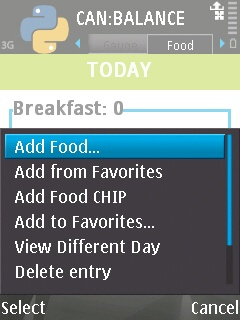
\includegraphics[ width =2.5cm ]{./images/cont1/fig4a}}
\label{fig:fib4a}
}
\subfloat[  ]{
\setlength\fboxsep{0pt}
\setlength\fboxrule{0.5pt}
\fbox{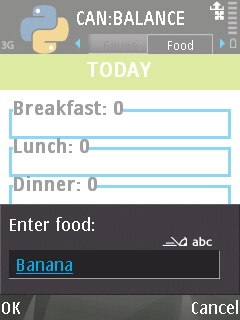
\includegraphics[ width  =2.5cm ]{./images/cont1/fig4b}}
\label{fig:fig4b}
}
\subfloat [  ]{
\setlength\fboxsep{0pt}
\setlength\fboxrule{0.5pt}
\fbox{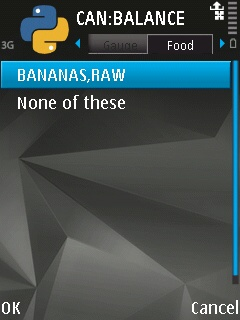
\includegraphics [ width  =2.5cm ]{./images/cont1/fig4c}}
\label{fig:fig4c}
}
\subfloat [  ]{
\setlength\fboxsep{0pt}
\setlength\fboxrule{0.5pt}
\fbox{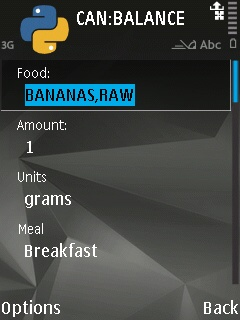
\includegraphics [ width  =2.5cm ]{./images/cont1/fig4d}}
\label{fig:fig4d}
}
\subfloat [  ]{
\setlength\fboxsep{0pt}
\setlength\fboxrule{0.5pt}
\fbox{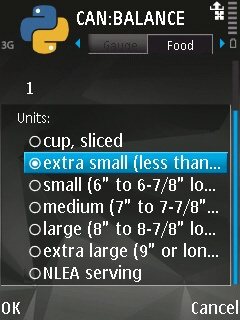
\includegraphics [ width  =2.5cm ]{./images/cont1/fig4e}}
\label{fig:fig4e}
}
\subfloat [  ]{
\setlength\fboxsep{0pt}
\setlength\fboxrule{0.5pt}
\fbox{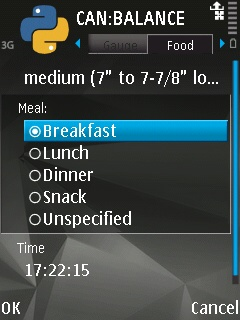
\includegraphics [ width  =2.5cm ]{./images/cont1/fig4f}}
\label{fig:fig4f}
}
\caption{Nokia prototype: Add known food}
\label{fig:fig4}
\end{center}
\end{figure}

Above (Figure 4), the screens depict the process of adding ``Banana'' to today's food diary. The user first selects ``Add Food'' from the menu, types in the term using T9 or multitap, and on submit, a list of foods that the user has entered before is shown. The user selects ``Banana, Raw'', and is shown a screen to modify the amounts and any timing information. By default, the USDA database has serving sizes in grams. Some entries have alternate serving sizes available. For ``Banana, Raw'', the serving sizes include ``cup, sliced'' and ``small (6'' to 6 7/8'' long). 

\begin{figure}[ t ]
\begin{center}
\subfloat[  ]{
\setlength\fboxsep{0pt}
\setlength\fboxrule{0.5pt}
\fbox{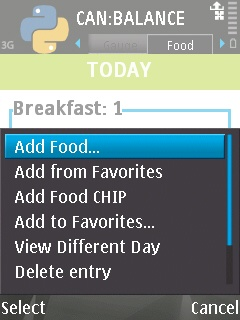
\includegraphics[ width =2.5cm ]{./images/cont1/fig5a}}
\label{fig:fig5a}
}
\subfloat[  ]{
\setlength\fboxsep{0pt}
\setlength\fboxrule{0.5pt}
\fbox{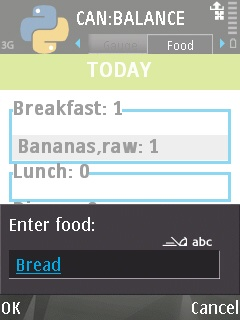
\includegraphics[ width  =2.5cm ]{./images/cont1/fig5b}}
\label{fig:fig5b}
}
\subfloat [  ]{
\setlength\fboxsep{0pt}
\setlength\fboxrule{0.5pt}
\fbox{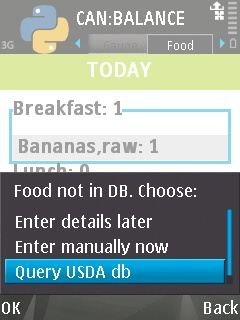
\includegraphics [ width  =2.5cm ]{./images/cont1/fig5c}}
\label{fig:fig5c}
}
\subfloat [  ]{
\setlength\fboxsep{0pt}
\setlength\fboxrule{0.5pt}
\fbox{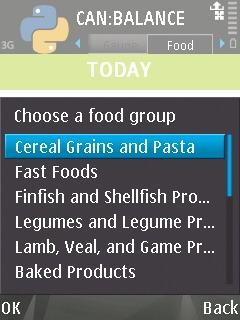
\includegraphics [ width  =2.5cm ]{./images/cont1/fig5d}}
\label{fig:fig5d}
}
\subfloat [  ]{
\setlength\fboxsep{0pt}
\setlength\fboxrule{0.5pt}
\fbox{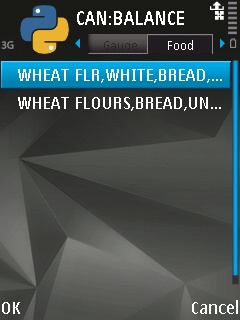
\includegraphics [ width  =2.5cm ]{./images/cont1/fig5e}}
\label{fig:fig5e}
}
\subfloat [  ]{
\setlength\fboxsep{0pt}
\setlength\fboxrule{0.5pt}
\fbox{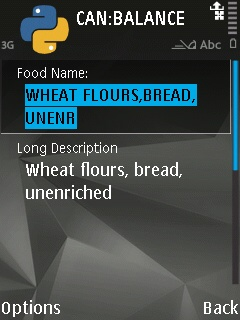
\includegraphics [ width  =2.5cm ]{./images/cont1/fig5f}}
\label{fig:fig5f}
}
\caption{Nokia prototype: Adding newly encountered (previously unused) food}
\label{fig:fig5}
\end{center}
\end{figure}

One primary goal for this project was for users to be able to quickly and accurately enter exactly how many calories they had consumed. This required finding the most appropriate, exact food and entering it in the exact amount, right after eating it. The process of finding food had to happen quickly to minimize interruption to the user. Queries to the entire food database took a long time to execute (this is described in further detail later), so to improve performance we separated the database into two separate databases: the entire USDA database and foods the user has entered before. The second database (``personal db'') reflects that many people have a relatively small number of foods they eat on a regular basis [ref]. When the user submits a search, the app first checks the personal db, which is fast because it's small. If there are no results, the user is asked whether they want to ``enter later'', ``enter manually'', or ``look up in USDA db''. The first option allows the user to bookmark the entry, since both the manual entry and USDA lookup are time consuming. The ``enter manually'' option provides a form for the user to make an entry based on the Nutrition Information panel required to be printed on all packaged foods. 

Figure 5 shows the process of entering a food (``bread'') that has not been used before; therefore it doesn't exist in the personal database. When ``bread'' is not found in the database, the user is given the option to look it up in the USDA database. When the query returns and contains foods that belong in more than one food group, it first lists the food groups to narrow down the list of possible choices. In this case, a search for ``bread'' resulted in foods in 14 food groups, and 3 pages of choices. Once the user chooses ``Cereal Grains and Pasta'', they can then choose the bread they ate, they can modify the name or details, and it is added to the personal database. The user can then specify the details needed to add it to the food diary. 

\subsection{Database Optimization and Querying}
One of the challenges of building dietary intake-tracking tools is identifying what kind of queries the user will make, what they expect the results to be, and generating a database query that provides the expected results from the nutrition database. 

Generating a query based on user input has performance implications, particularly when working with text. Queries on a string column are slower than other data types, and searching for strings with wildcards further degrades the response time. 

In the BALANCE software, a user provides a basic query, and the software generates a query based on that user input. Each word the user provides becomes a predicate in the query. This approach results in queries that are known to have poor performance, but this is necessary to account for the ordering of relevant terms in the database. Table [ref] gives some examples of food terms that a user might enter, and some example entries in the database.  
% Table generated by Excel2LaTeX from sheet 'Sheet1'
\begin{table}[htbp]
  \centering
  \caption{Add caption}
    \begin{tabular}{p
{2cm}p{3in}l}
    \toprule
    \textbf{User Search Request} & \textbf{Query WHERE clause} & \textbf{Example matches from database} \\
    \midrule
    \multirow{4}[2]{*}{cheese
} & \multirow{4}[2]{*}{
LIKE �*cheese*� 
} & Cheese, Cheddar \\
          &       & Cheese, Cream \\
          &       & Bagel with Cream Cheese \\
          &       & Pizza, Cheese and Pepperoni \\
    \multirow{2}[2]{*}{cream cheese} & \multirow{2}[2]{*}{LIKE �*cream*� AND LIKE �*cheese*�} & Cheese, Cream \\
          &       & Bagel with Cream Cheese \\
    \bottomrule
    \end{tabular}%
  \label{tab:table1}%
\end{table}%


\subsection{Observations}
The first prototype of the BALANCE software helped us to identify unanticipated difficulties. In this section, I describe the problems we observed. The problems generally relate to the process of finding and choosing a food for the food diary. A summary list is shown below, and I further describe each one: 
\begin{enumerate*}
\item Text entry was too hard with 12-key keypad. 
\item It took too long to search due to poor db performance. 
\item It was difficult to find and choose a specific food. 
\begin{itemize*}
\item Using Food Class to filter search results. 
\item Long names that didn't fit on the screen. 
\item No entry for commonly prepared foods. 
\item For some foods, many variations to choose from. 
\end{itemize*}

\end{enumerate*}

\subsubsection{Text Entry Was Too Hard}
The 12-key keypad required users to use multi-tap or T9 to enter the names of food they have eaten. This is very difficult to do for foods with long names. The decision users encountered every time they wanted to enter a food was whether to commit to typing in a long, detailed food name that is likely to generate fewer food choices to choose from, or type in a short food name which resulted in many responses. 

\textbf {Recommendation: } To appeal to less tech-savvy consumers, provide a more comfortable means of text input. 

\subsubsection{Too Long To Search}
As discussed above, user input is converted into a query that is known to have poor performance. This is partly due to a mismatch between what the user wants to search for (``cream cheese'') and how it may be stored in the database (``cheese, cream'' or ``bagel, with cream cheese''). It's important that the software returns all of the results. 

This concern is primarily due to the limited resources on the mobile phone. The database available on the mobile platform has reduced capabilities as compared to those available on a desktop or in a high performance computing environment, and the limited processing power of the device magnifies the limitations of the database. 

\textbf {Recommendation:} Faster hardware, improve the filtering process.
 
\subsubsection{It Was Difficult To Find And Choose A Food}
After entering a food query and waiting for the search to return, a user needs to choose the desired food from all of the results. 
Using Food Class to filter search results. As noted earlier, if the results are from just one Food Class, the entire list of results is immediately shown. If there are results in multiple Food Classes, the list of Food Classes is shown to allow the user to choose the most appropriate. To find the target food, the user must choose from a potentially long list of Food Classes (the results for the query ``Bread'' include 16 Food Classes). Some of the food classes are difficult to distinguish. For example, the Food Classes for ``Bread'' includes both ``Cereal Grains and Pasta'' and ``Baked Goods''. This requires the user to make a decision, and users unfamiliar with the Food Classes aren't sure which to choose. 

\textbf{Recommendation: }Don't force the user to think about arbitrary Food Classes. Provide guidance about what each Food Class represents. Provide some ``teasers'' or a few items of that Food Class to demonstrate what kinds of foods it contains. 

\paragraph{Long names don't fit on the screen.}
The USDA database contains food descriptions that are long and descriptive. For example, a typical entry for the query ``Steak'' is ``Beef, short loin, porterhouse steak, separable lean and fat, trimmed to 1/4'' fat, USDA choice, raw''.  The alternative ``short'' description is a similar entry using defined abbreviations: ``Beef, shrt loin,prtrhs steak,ln,1/4'' fat,usda choic,raw''. Neither of these descriptions display well on the small screen size of the target device. If they are displayed one entry per line in a font that is comfortable to read, not enough words are shown to distinguish one entry from another. If the description is shown on multiple lines, only one or two entries can be shown at a time. Forcing the user to select one to see more detail and then returning to the list screen is time consuming and frustrating. 
 
\begin{figure}[ t ]
\begin{center}

\setlength\fboxsep{0pt}
\setlength\fboxrule{0.5pt}
\fbox{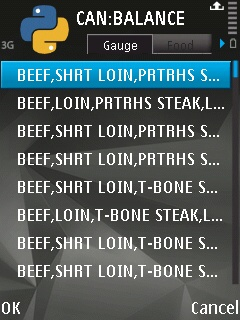
\includegraphics [ width  =2.5cm ]{./images/cont1/fig6}}

\caption{Nokia prototype: 'Steak' results}
\label{fig:fig6}
\end{center}
\end{figure}

\textbf {Recommendation: }Use a larger display with higher resolution. Use a database that has more useful short descriptions. Structure the database to provide a short ``food name'', a short description, and a detailed description. 
No entries for common prepared foods. One of the drawbacks of the USDA database is that it did not include many prepared foods, such as those purchased at a grocery store or restaurant. The database contains food entries from only 60 manufacturers, which include some of the major food manufacturers in the US (Burger King, Kellogg, Nestle, McDonalds). However, users expect that if they can purchase a food (ie, it has a UPC code), then it will be in the database. 

\textbf{ Recommendation:} Choose a database that includes a more comprehensive list of prepared foods. 

For some foods, many items to choose from.  For some foods, there are many entries. For example, a query for ``Cheese'' in the ``Dairy and Egg Products'' Food Class has 44 entries. The cheese entries are somewhat reasonable: blue, brick, brie, camembert, caraway, cheddar, etc. Some may be unfamiliar to a user, but they are clearly different and possibly significantly different. The results for ``Porterhouse'' (steak) are not so clearly different, however: 
\begin{itemize*}
\item Beef, short loin, porterhouse steak, separable lean and fat, trimmed to 0'' fat, all grades, cooked, broiled
\item Beef, short loin, porterhouse steak, separable lean and fat, trimmed to 0'' fat, USDA choice, cooked, broiled
\item Beef, short loin, porterhouse steak, separable lean and fat, trimmed to 0'' fat, USDA select, cooked, broiled
\item Beef, short loin, porterhouse steak, separable lean only, trimmed to 0'' fat,  all grades, cooked, broiled
\item Beef, short loin, porterhouse steak, separable lean only, trimmed to 0'' fat, USDA choice, cooked, broiled
\item Beef, short loin, porterhouse steak, separable lean only, trimmed to 0'' fat, USDA select, cooked, broiled
\end{itemize*}

Users are confused about how to choose which one they should enter, and wonder whether the difference between all these entries really matters. Additionally, the amount of distinguishing detail for this entry makes them wonder if they should be capturing that amount of detail for all of the foods they enter. This compounds the previous problem of not being able to find prepared foods. 

\textbf Recommendation: \textbf Use a database that was designed for use by a consumer rather than an expert. 

Overall, the process to add food to the food diary is just too long, due to all of the factors described in detail above. For the BALANCE project, it was important that users are able to enter foods quickly, so that they are able to enter food throughout the day and ensure the fuel-gauge visualization is properly updated. 

\subsection{Discussion}
This prototype experience made us more aware of the inherent challenges around designing and developing a food diary for a mobile phone. The challenges are due partly to the database, and partly from using a device with limited interaction modes to navigate a challenging data environment. The population we were targeting is a general population, not necessarily very comfortable entering text via multitap/T9; the challenge of text entry magnifies the problem of querying the database and navigating the results. 

One conclusion from this process was to use a different mobile phone. The original Symbian S60 device was much friendlier to use and more powerful than previous smartphones, but the general population had not yet much experience with smartphones, and this was the target population for the project. Text entry was one of the biggest barriers: the 12-key keypad with multitap or T9 input was not comfortable to most consumers. 

The database negatively impacted the navigation and performance. Database entries were not well suited to the mobile phone display, and the query process on the device was too slow to be acceptable. It is also necessary to have more popularly available packaged/prepared foods, although some of the closely related foods could be collapsed. The importance of the database in self-monitoring or dietary assessment is outlined in [ref][Stumbo08]. Indeed, they state ``Mastery of computerized dietary assessment requires an understanding of the database in terms of the naming conventions, the search strategy for finding foods, and data completeness for generic and brand-name foods.'' This is consistent with our experiences. 

\section{Food Databases}
There are conflicting requirements for the food database. The database needs to be quick to search (small), yet have the foods that people eat and are looking for (complete/large). It also needs to be able to distinguish between similar items, and use terminology that is familiar to the target user population. Grouping into friendly and familiar food groups or classes will help users to find food in the database by providing data to filter on or browse. Providing useful, appropriate serving sizes is another helpful feature. For example, Coca Cola should have commonly available serving sizes to choose from, such as a 12-oz can, a 20-oz bottle, or a 16-oz cup, even if the typical/official serving size is 8 oz. 

The history of food databases might be helpful in understanding the characteristics of the databases. Generally, food databases are used by professionals, experts in food service, preparation, and evaluation. Hospitals, nursing homes, and other medical facilities use food databases to make sure that patients are fed properly, within the constraints they might have. They generate menus for days, weeks and months, using the database to ensure proper nutrition for all recipients. Nutritionists and registered dieticians use commercial food databases to work with clients who have certain dietary constraints-either to look up foods that an individual ate and evaluate their diet overall, or to generate a meal plan for an individual and provide detailed information about it. Organizations such as daycares, schools and prisons (especially those that get government funding) use the food databases to ensure that they meet governmental guidelines. Food manufacturers use food databases to generate Nutrition Facts labels for their products. 

For the tasks I've outlined above, the end user of the database is an expert who is familiar with food systems, organization, and terminology. The user has been trained, and uses the database on a regular basis. Increasingly, food databases have been made available to the general population, usually in the form of a consumer tool. 

Table 2 provides some information on two databases: the USDA (SR21) database we used for the first prototype, and the NutritionistPro Knowledge Base that we used for the next version of the software. 

% Table generated by Excel2LaTeX from sheet 'Sheet2'
\begin{table}[htbp]
  \centering
  \caption{Comparing nutrition databases}
    \begin{tabular}{p{2in}p{2in}p{2in}}
    \toprule
    \textbf{} & \textbf{USDA} & \textbf{NutritionistPro Knowledge Base} \\
    \midrule
    \textbf{Version} & SR21 (Sept 2008) & V44 (Fall, 2009) \\
    \textbf{File Size (Access db)} & 16.5Mb & 135Mb \\
    \textbf{Number of foods} & 7,412 & 39,194 \\
    \textbf{Number of food servings (types?)} & 13,087 (num records in the �Weight� table)  & 46,722 (num records in tblFoodServingTypes) \\
    \textbf{Number of unique serving type descriptions} & 1700  & 5087 \\
    \textbf{Number of Manufacturers} & 60    & 592 \\
    \textbf{Num Recipes} &       & 783 \\
    \textbf{Food Groups} & 24    & 369 (Food Classes�hierarchical) \\
    \textbf{Number of nutrients } & 140   & 90 \\
    \bottomrule
    \end{tabular}%
  \label{tab:table2}%
\end{table}%

 
\section{Food Diary: Iterative Design And Evaluation}
In this section, I describe the design and features of the food diary portion of the overall BALANCE project. The challenges identified in the previous section informed the decision to move to a Windows Mobile platform and adopt a commercially available nutrition database to drive the food diary. The combination of the paper prototype user study and Symbian implementation informed the new design on the Windows Mobile platform, and the final design was informed by an iterative, user-centered evaluation process. 

Focus groups of 4-5 participants provided user feedback in the design and development process. We convened 5 focus groups over a 7 month period. Participants were given a mobile phone running the food diary software, and asked to track what they eat for three days prior to the focus group. After the three days of tracking and before the focus group, participants were asked to complete 2 usability questionnaires (CSUQ and MPUQ, [ref]). The focus group was moderated by a team member, and topics focused on what the participants liked, what worked and didn't work, and features they would like to see added. Details are in Appendix [ref]. Feedback from the participants in the focus groups provided input to the design and development of the next software iteration. 
We used two metrics to evaluate the overall progress of the iterative process. First, we analyzed usability questionnaire responses over time. These did not show a significant improvement of the usability of the food diary software overall. The other measure of progress we considered was the time between when a participant ate a food, and when they entered it in the food diary. We hypothesized that this time would decrease as the food diary improved. This also did not show a significant improvement of the food diary. Details of the analysis are provided in [ref], and I discuss the use of these metrics later in this section, as well as in Chapter [x] [ref]. 

\subsection{Overall Design}
The final version of the BALANCE software ran on a Windows Mobile 6.1 Professional device. We chose this device because it had a large display, a touch screen, and a slide-out QWERTY keyboard. Text input can be done either via the physical QWERTY keyboard or with the ``soft input panel'', on-screen keyboard. We used the NutritionistPro Knowledge Base for the food diary. 

\subsubsection{Food Diary Software}
The primary task for this software is to enable users to find a food that they've eaten from a database, specify how much of it they ate, and save a record of it. 

\begin{figure}[ t ]
\begin{center}
\subfloat[  ]{
\setlength\fboxsep{0pt}
\setlength\fboxrule{0.5pt}
\fbox{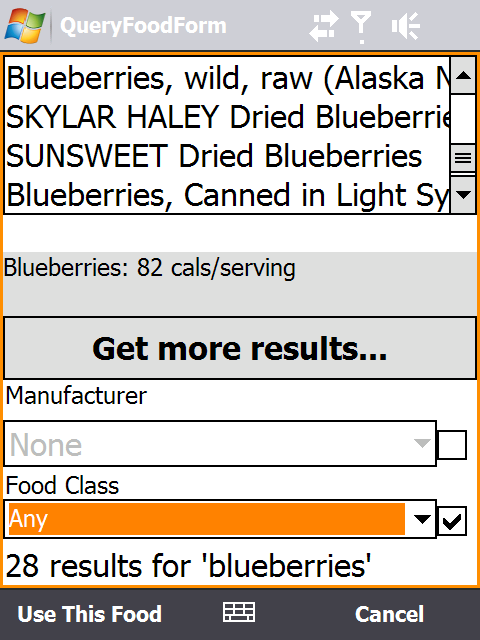
\includegraphics[ width =2.5cm ]{./images/cont1/fig7a}}
\label{fig:fig7a}
}
\subfloat[  ]{
\setlength\fboxsep{0pt}
\setlength\fboxrule{0.5pt}
\fbox{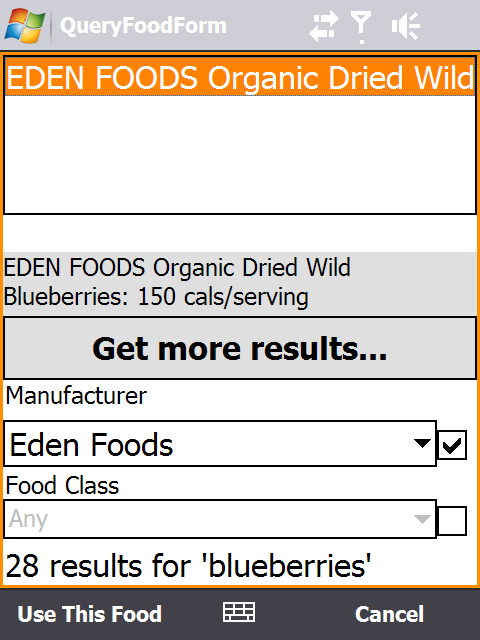
\includegraphics[ width  =2.5cm ]{./images/cont1/fig7b}}
\label{fig:fig7b}
}
\subfloat [  ]{
\setlength\fboxsep{0pt}
\setlength\fboxrule{0.5pt}
\fbox{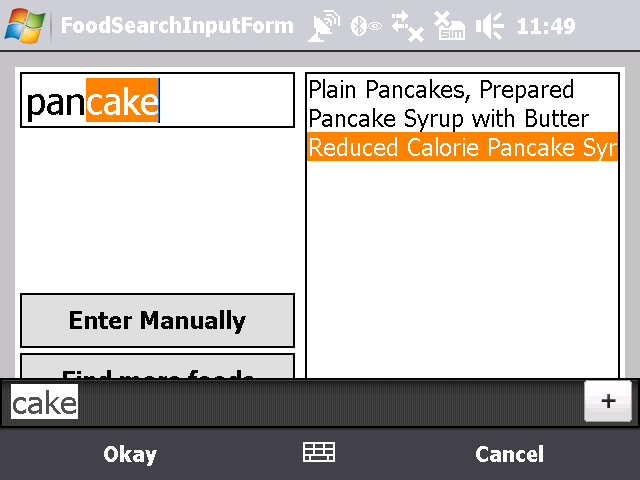
\includegraphics [ width  =2.5cm ]{./images/cont1/fig7c}}
\label{fig:fig7c}
}
\subfloat [  ]{
\setlength\fboxsep{0pt}
\setlength\fboxrule{0.5pt}
\fbox{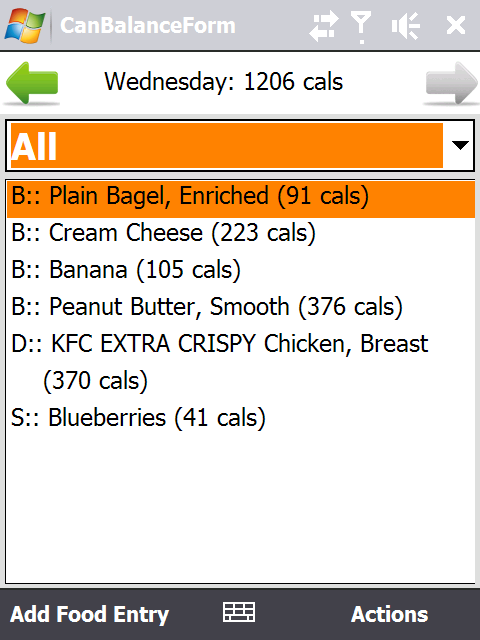
\includegraphics [ width  =2.5cm ]{./images/cont1/fig7d}}
\label{fig:fig7d}
}

\caption{WinMobile Food diary}
\label{fig:fig7}
\end{center}
\end{figure}

Figure 7 shows a walkthrough of the add food process. The application starts with a list of food that's been eaten today. The ``Add Food'' button displays a screen that allows the user to start typing an entry. As the user types, a list of common or recently eaten foods populates the display. If the user sees what they want, they can select it, or choose to ``Enter Manually'' (create a new entry based on the Nutrition Information label on the package), or ``Find more'', which searches the entire food database (a). This list can be filtered by manufacturer and food class (b). Once a food is selected, the user specifies what time they ate the food, which meal it should be counted with, and how much of it they ate (c). The entry is then saved and shown on the daily food list (d). 

\subsection{Selected Features and Feedback}
Throughout the iterative design process, we aimed to improve the existing functionality and add features as necessary. In this section, I describe a couple of the features that evolved based on user feedback. 

\subsubsection{Touch Friendly Screen Design }
\begin{figure}[ t ]
\begin{center}
\subfloat[  ]{
\setlength\fboxsep{0pt}
\setlength\fboxrule{0.5pt}
\fbox{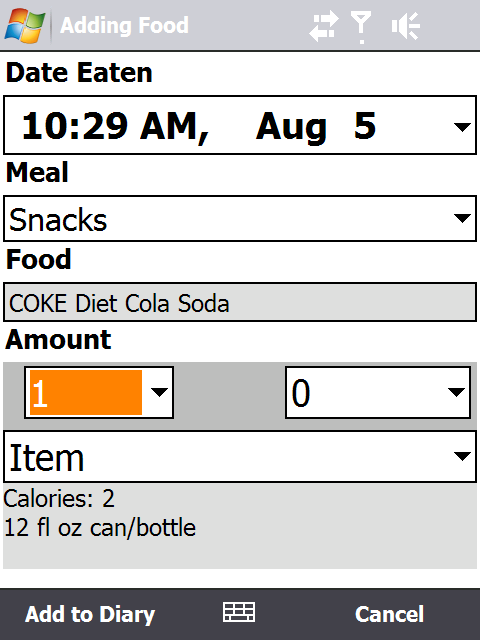
\includegraphics[ width =2.5cm ]{./images/cont1/fig8a}}
\label{fig:fig8a}
}
\subfloat[  ]{
\setlength\fboxsep{0pt}
\setlength\fboxrule{0.5pt}
\fbox{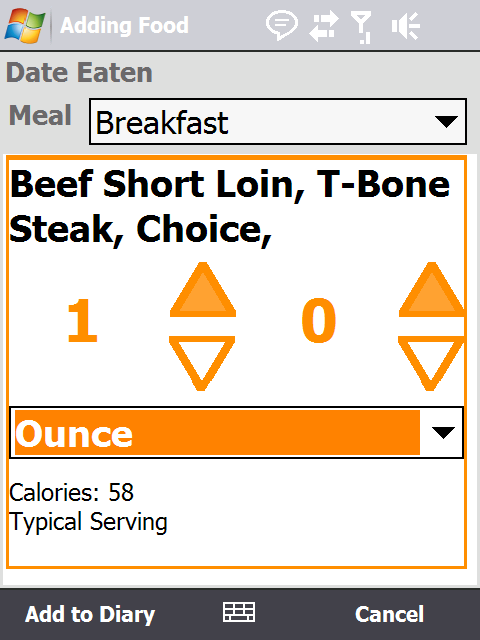
\includegraphics[ width  =2.5cm ]{./images/cont1/fig8b}}
\label{fig:fig8b}
}
\subfloat [  ]{
\setlength\fboxsep{0pt}
\setlength\fboxrule{0.5pt}
\fbox{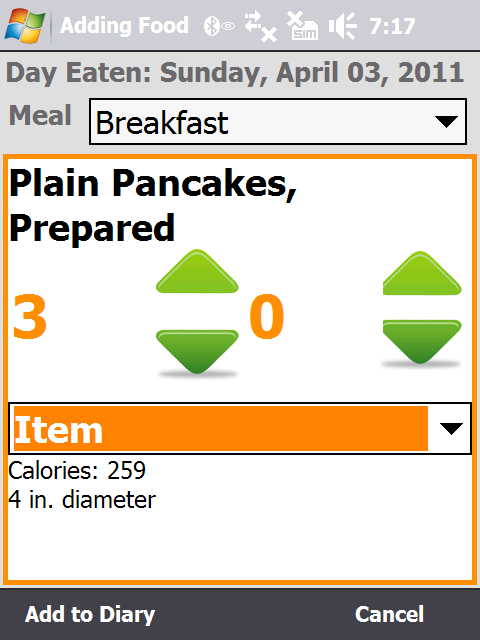
\includegraphics [ width  =2.5cm ]{./images/cont1/fig8c}}
\label{fig:fig8c}
}
\caption{Evolution of serving size specification}
\label{fig:fig8}
\end{center}
\end{figure}
One of the reasons we chose the final device was for its touch-sensitive screen. To improve the time it takes to create a food entry, the items on the screen were displayed big enough to be selected by a finger/fingernail. However, early in the feedback process, users reported that they didn't like the stylus-it was too small to hold comfortably, there was fear around losing it, and it was time consuming to take it out and put it back. Therefore, one change we made was to replace the traditional WinMobile UI widgets with custom graphical widgets that looked friendlier to touch. Users remarked on the ``friendliness'' and ``cheeriness'' of the new widgets. 

\subsubsection{Create New Food Database Entry}
The NutritionistPro database contained many foods, but users still reported encountering foods that were not in the database. This resulted in the ability to add a new food to the database, using information from the Nutrition Facts label all packaged foods are required to have. After the entry is created, it shows up in the quick-search results with other common and recently used foods. 
 
\begin{figure}[ t ]
\begin{center}

\setlength\fboxsep{0pt}
\setlength\fboxrule{0.5pt}
\fbox{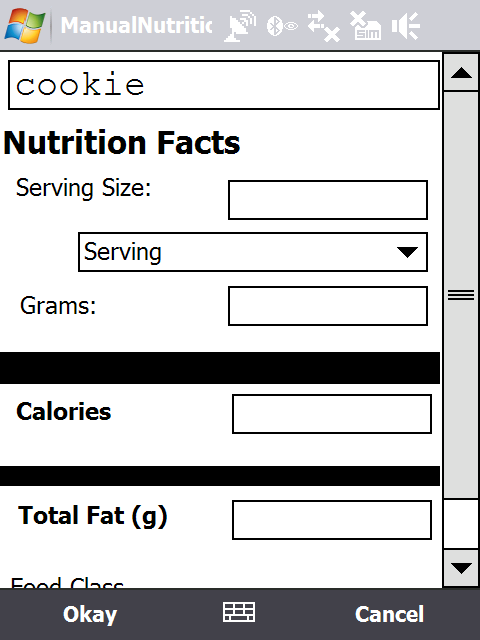
\includegraphics[ width =2.5cm ]{./images/cont1/fig9}}


\caption{Add new entry (manual) to food diary}
\label{fig:fig9}
\end{center}
\end{figure}

\subsubsection{Favorite Meals}
Focus group participants repeatedly [ref] asked for the ability to bookmark favorite foods, and specify combinations that were commonly eaten together as a meal. We make a distinction between a recipe and a meal: A meal is a group of foods commonly eaten together, such as coffee and a donut, which might be a common order at one's favorite coffee shop, or the typical sandwich one makes for lunch. A recipe consists of a bunch of foods combined, usually to make multiple servings. For this version of the software, we did not implement the recipe-creation feature, but did implement the ability to specify favorite foods and meals, as shown below (Figure 10). 

\begin{figure}[ t ]
\begin{center}
\subfloat[  ]{
\setlength\fboxsep{0pt}
\setlength\fboxrule{0.5pt}
\fbox{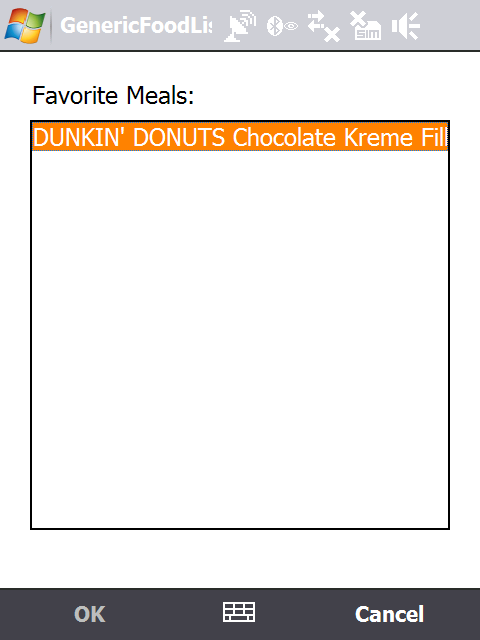
\includegraphics[ width =2.5cm ]{./images/cont1/fig10a}}
\label{fig:fig10a}
}
\subfloat[  ]{
\setlength\fboxsep{0pt}
\setlength\fboxrule{0.5pt}
\fbox{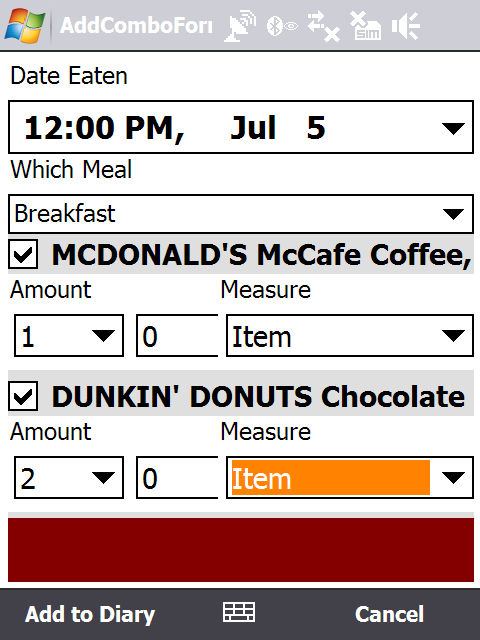
\includegraphics[ width  =2.5cm ]{./images/cont1/fig10b}}
\label{fig:fig10b}
}
\subfloat [  ]{
\setlength\fboxsep{0pt}
\setlength\fboxrule{0.5pt}
\fbox{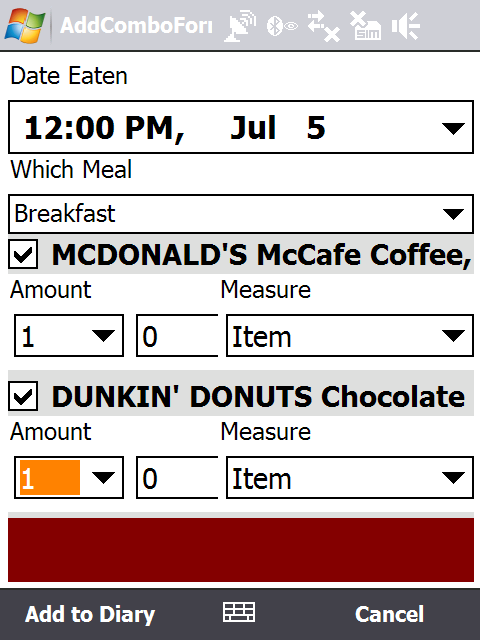
\includegraphics [ width  =2.5cm ]{./images/cont1/fig10c}}
\label{fig:fig10c}
}
\subfloat [  ]{
\setlength\fboxsep{0pt}
\setlength\fboxrule{0.5pt}
\fbox{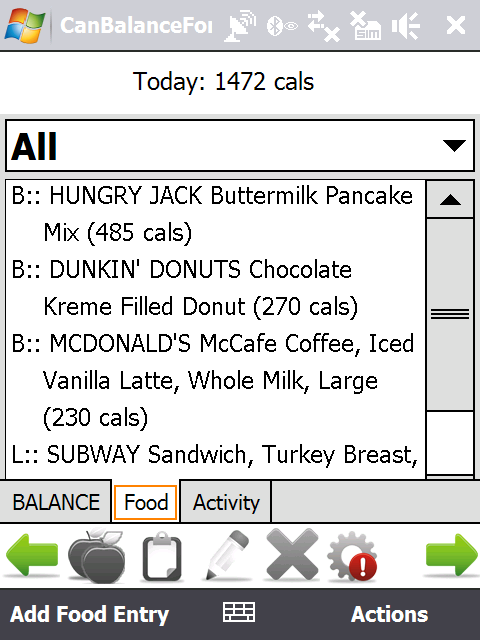
\includegraphics [ width  =2.5cm ]{./images/cont1/fig10d}}
\label{fig:fig10d}
}

\caption{Favorite meals walkthrough}
\label{fig:fig10}
\end{center}
\end{figure}

\subsection{Database Query Details}
Adopting the commercially available NutritionistPro database resulted in a much larger number of foods available to the user. While the USDA database had the user challenge of making it difficult to distinguish between many similar unprocessed foods and relatively few processed/manufactured foods, the NutritionistPro database had many more processed and manufactured foods to choose from, which users sometimes found overwhelming. 

In this section, I describe some of the ways we tried to make the query process more user friendly. Rather than describe all the possible improvements we considered, I focus on the final implementation. 

One weakness of the database supported on the Windows Mobile platform (Sql Server CE) is that it doesn't support full text search (FTS). When FTS is available on a database, queries can be made that reflect linguistic characteristics of a given language (such as English). With a FTS capability, one can easily query  not just for a word or a phrase, but a word or a phrase that starts with given text (prefix), inflectional forms of a word (for example, foot or feet), a word or phrase close to another word or phrase, or a synonymous term. This is valuable in the case of food diaries, because from the user's perspective it's sometimes unclear whether the food diary will have ``Potatoes, Mashed'' or ``Mashed Potatoes'' as an entry. Additionally, consumers in general are familiar with search strategies that employed FTS, whether or not they know enough about it to specify it exactly. Users are able to articulate is that a particular search function ``just knows what I'm looking for'' and ``does the right thing'', linguistically-a search for ``potatoes'' also yields results with ``potato''. 

In addition to the lack of linguistic support that FTS provides when searching text in a database, speed is a consideration. The alternative to FTS is a LIKE query based on character patterns. A LIKE query against millions of rows of text data can take minutes to return; whereas a FTS query can take only seconds or less against the same data, depending on the number of rows that are returned (due to the pre-built index).

We tried to overcome the lack of free-text search on the database by being smart about the queries we generated. However, the more complex a query became, the longer the time to respond, even if the results were ``better''.  In general, our approach favored returning better results faster, rather than minimizing the size of the database. Storage was cheap: we could easily add a larger memory card to the device, but we couldn't improve the processor. 

To improve the query time and search process, we implemented a ``poor man's predictive search''. As mentioned above, the system contained two food databases: the large, complete NutritionistPro database, and a smaller, personalized personal database. The personal database was initially seeded with foods marked as ``common'' or ``generic'' in the NutritionistPro database. To improve the responsiveness, there was a table in the personal database that contained the first 3 letters of all words in the food name, description and manufacturer name associated with a food entry. When the user starts typing to search for a food name, after 3 characters are entered, a results box is generated based on an exact string match from that table. As the user continues typing, the list of results is filtered based on that text. If a desired food is not found, the user can ``Find More'', which ends up performing the longer LIKE query on the NutritionistPro database. When a food is selected from the NutritionistPro database and entered into the food diary, it is also stored in the personal database, and the prefix table is updated. This adds time to the process, but this time is negligible to the time required for the NutritionistPro query. 

\subsection{Metrics}

In this section, I want to talk about the metrics we used to guide the development and evaluation of the software. Specifically, I want to review what we used, how they worked, why they failed, and propose alternate metrics to collect during the final evaluation. 

One way we attempted to quantify the success of the software by measuring the time between when a food was eaten and when it was entered into the diary. This metric didn't show any significant improvement, but it did highlight important information about how the software is used. In the focus group discussions, participants volunteered that they didn't enter food throughout the day, and weren't likely to. Multiple reasons were given for this: sometimes it was just that the person was too busy and couldn't take the time, and sometimes it was just easier to do it all at once later in the day. Some participants noted that they took advantage of [pockets of free time] such as when waiting at the bus to review and enter their food. This gives us some insight, but it's still unclear whether they won't enter it at the time because the software is bad, or if they won't enter it the time because it's an inherently tedious process, or due to external influences. 

This experience highlighted the importance of identifying appropriate metrics for evaluating food diaries on cell phones, reflecting both usability/how the software is being used and domain success-whether people are able to achieve the stated goal (capturing the right number of calories by identifying all the foods one ate). 

\section{Validating BALANCE}
The final BALANCE validation combined all key components of the project: the MSB device for calorie expenditure calculation and the mobile phone with the visualization, food diary and activity diary software. Participants were asked to carry the mobile phone and MSB for 4 days. They were asked to enter all food and drink consumed (except water), and manually enter the activity that the MSB didn't track. They were asked to record on days 1, 3 and 4, but on the second day they only performed a 24-hr recall of what they ate on the first day. They completed a post-use questionnaire intended to identify useful features, and completed an activity questionnaire. See Snively[ref] for more details. 

\subsection{Final BALANCE Software}
Up until this point, the discussion has focused on the design and development of the food diary and visualization components of the BALANCE project, independently. As mentioned earlier, the entire project consists of the feedback visualization, food diary, activity diary, and activity sensing component (MSB) combined together. In this section, describe the activity portion of the system. 
The activity diary (shown in [ref]) shows both activities entered by the user and activity information detected by the MSB. The user is responsible for entering activity not detected by the MSB, such as swimming or vigorous (?) sports. The activity database is based on the Physical Activity Compendium [ref]. 

\begin{figure}[ t ]
\begin{center}
\subfloat[  ]{
\setlength\fboxsep{0pt}
\setlength\fboxrule{0.5pt}
\fbox{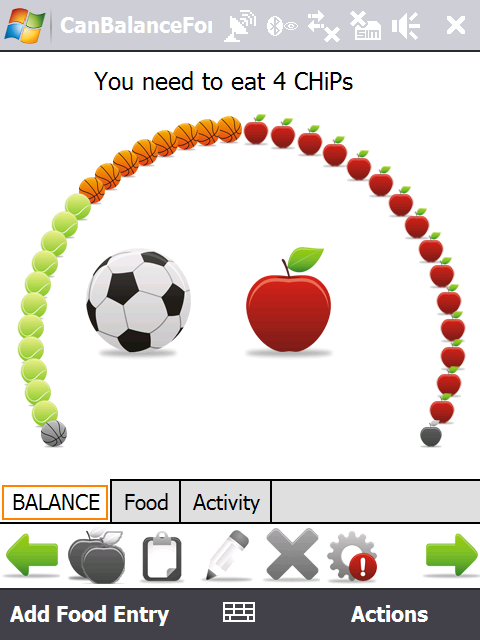
\includegraphics[ width =2.5cm ]{./images/cont1/fig11a}}
\label{fig:fig11a}
}
\subfloat[  ]{
\setlength\fboxsep{0pt}
\setlength\fboxrule{0.5pt}
\fbox{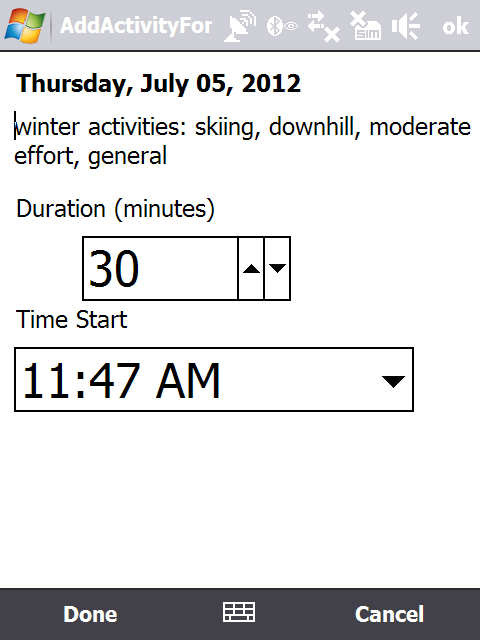
\includegraphics[ width  =2.5cm ]{./images/cont1/fig11b}}
\label{fig:fig11b}
}
\subfloat [  ]{
\setlength\fboxsep{0pt}
\setlength\fboxrule{0.5pt}
\fbox{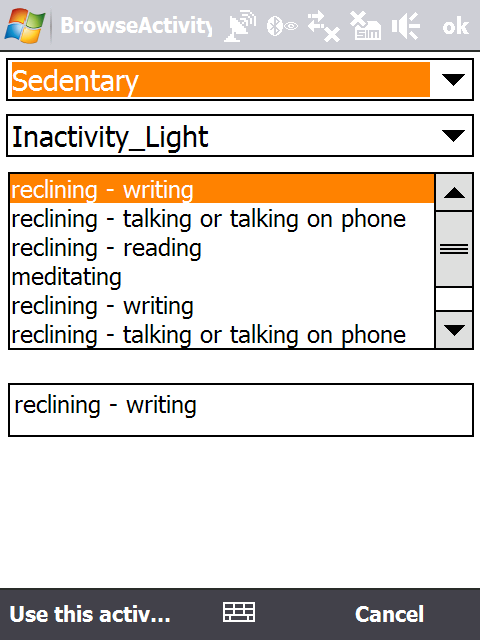
\includegraphics [ width  =2.5cm ]{./images/cont1/fig11c}}
\label{fig:fig11c}
}
\subfloat [  ]{
\setlength\fboxsep{0pt}
\setlength\fboxrule{0.5pt}
\fbox{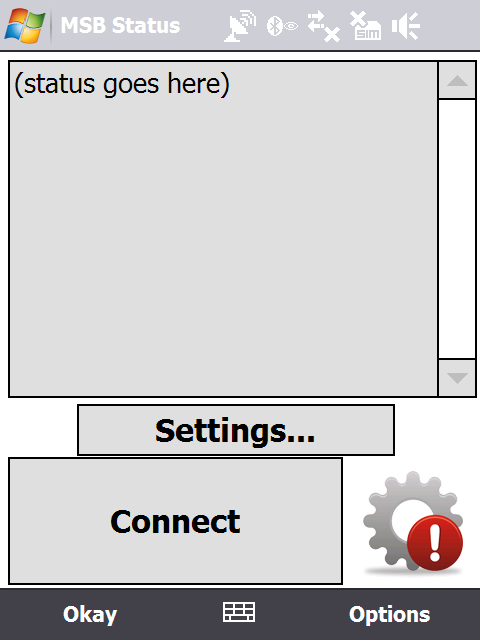
\includegraphics [ width  =2.5cm ]{./images/cont1/fig11d}}
\label{fig:fig11d}
}

\caption{Final BALANCE software walkthrough}
\label{fig:fig11}
\end{center}
\end{figure}

The pager-sized MSB is worn on the user's hip, and is connected to the phone via Bluetooth. The interface supports connecting to and communicating with the device, displaying information about the sensed activities. The software also monitors the connection and notifies the user if the connection breaks. 


\subsection{24-hr recall software. }
A 24-hr recall is a process in which a trained researcher works with the participant to identify all the foods that the person ate in the past 24 hrs. Part of the BALANCE validation required identifying how correctly and completely the user entered the food they ate into the mobile phone food diary. To do this, participants were asked to complete a 24-hr recall for the first day of their participation. The protocol is designed to elicit information from the person without ``planting false memories'', as well as identify commonly forgotten foods. 

\begin{figure}[ t ]
\begin{center}

\setlength\fboxsep{0pt}
\setlength\fboxrule{0.5pt}
\fbox{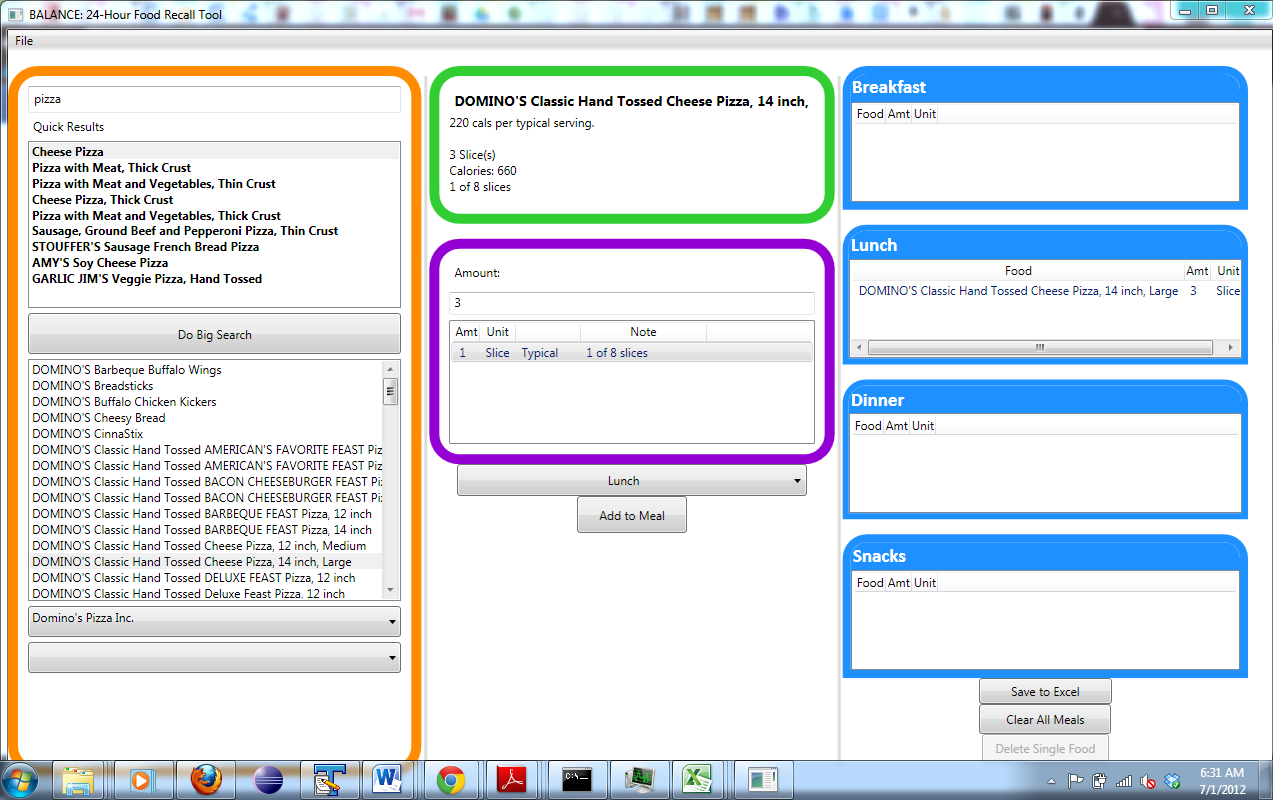
\includegraphics[ width =10cm ]{./images/cont1/fig12}}

\caption{WinMobile Food diary}
\label{fig:fig12}

\end{center}
\end{figure}

This process required a tool for the researcher to access the same food database in the same manner that the participants did. We developed a desktop version of the food diary app to support this task. 

\subsection{Metrics}
As mentioned above, our evaluation of the iterative design process was unsatisfactory overall. A secondary goal of this validation phase was to collect more metrics about how the software was used, to try to evaluate or generate some ideas for further research on metrics that may be more informative indicators of the use of the software. 

In this section, I describe the metrics we collected, as well as the results. I also address how the reported metric results could help better understand the final validation, which identified a discrepancy between calories entered into the food diary and calories determined via the 24-hr recall. In Chapter [ref], I refer back to this in the larger context of evaluating the use of food diaries. 
One thing that informs some of these choices is the HCI/Persuasive Tech research community. Technology researchers working in the space of health and wellness have long acknowledged that actual behavior change cannot be the primary measure of success for evaluating tools to help support behavior change. Early prototypes and investigations into the space will need other measures to indicate whether the tool is developing in the right direction or not. In this vein, we are increasingly focusing on ``indicators of engagement'', which , loosely defined, are metrics that reflect how engaged an individual is with a particular tool. The reasoning is that the higher the level of engagement (and the more sustained the engagement), the greater the chance for behavior change. That said, no research has clearly shown how useful different indicators of engagement are. 

In this section, I report how different metrics change over the five days following the start of the study, per participant. Days 1-4 reflect active participation in the study, while day 5 reflects any modifications to the earlier data. To compare and characterize change in the metrics over time, each study day is broken into 6 4-hr periods, ``Early morning'' (12-4am) through ``Night'' (8-12pm). No distinction is made between weekends and weekdays. 

\subsubsection{App Starts Over Time}
The first metrics of engagement we consider is how many times the user starts the application. Even if they don't do anything with the app, starting the app usually indicates that the user is thinking about the app. In the case of the BALANCE software, starting the app could reflect a number of things, including that the user just ate and is planning to make an entry, planning to eat and looking up an calorie values, is glancing at the visualization to assess progress in the middle of the day, or is planning to enter a forgotten entry from earlier in the day. 

A common descriptive metric to report is the mean number of app starts or entries per day, per participant {``participants made an average of 3.26 entries per day''}[ref][examples-Wellness Diary]. For BALANCE, that's not informative enough. This project in particular puts value on the user being engaged with the software throughout the day. We want to know if people are thinking about it consistently throughout a day, and how that pattern changes over time. 
For each participant, we calculated how many times the app was started in every 4-hr time period after their start of the study (midnight of Day 1). Reviewing the data revealed that some people started the app throughout the day, while others only started it once a day, and sometimes people didn't start it at all. Figure 13 shows the counts of participants whose data reflected these behaviors. 
\begin{figure}[ t ]
\begin{center}

\setlength\fboxsep{0pt}
\setlength\fboxrule{0.5pt}
\fbox{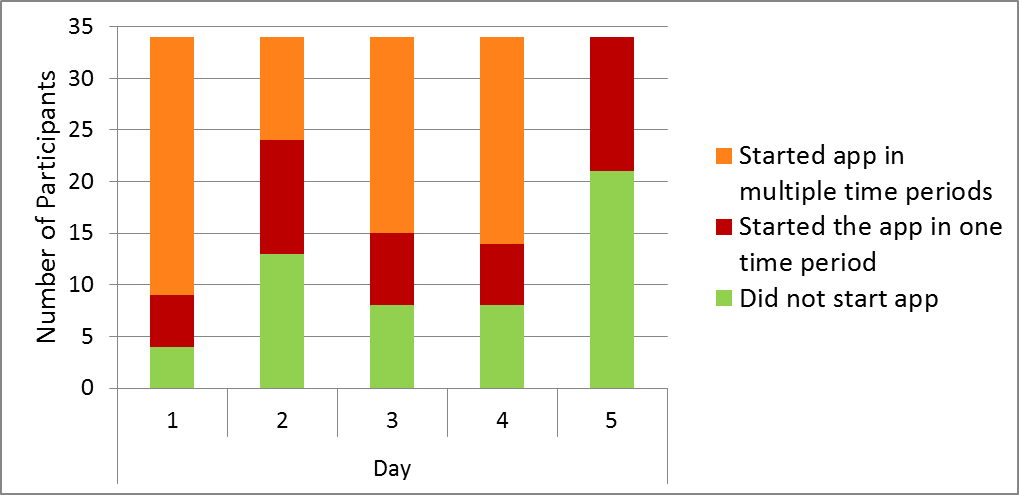
\includegraphics[ width =10cm ]{./images/cont1/chart13}}

\caption{App start patterns over the days }
\label{fig:chart13}

\end{center}
\end{figure}

If everyone used the software the way we intended them to, the above chart would show 34 people starting the app multiple times throughout the day (blue) on days 1, 3, and 4 (the days of the study when they are entering their food). However, we see that while many people started the app consistently on the days 1, 3, and 4, it wasn't everyone, and that number decreased on days 3 and 4. From looking closer at the raw data, we saw that 11 people displayed the desired pattern, which indicated that they used the app as requested. 13 people had at least one day (of days 1, 3, or 4) where they didn't start the app at all, and 5 had 2 days when they didn't start the app at all. 2 people consistently started the app 1 time/day for the duration of the study. 

One problem with this calculation is that not starting the app doesn't necessarily mean that a participant wasn't *using* the app consistently throughout the study. 2 participants never started the app throughout the study period, but still had valid entries. This can be explained that participants treated the phone as a special device only used to enter their food. Since participants were asked to carry a separate device rather than use their personal phone, they weren't using the device for anything else, and likely had no reason to ``quit'' and re-start the app. 

\textbf{What does this mean for the validation discrepancy?} This data indicate that for the most part, participants were starting the application periodically through the day. This meant that the discrepancy is probably not due to people forgetting about the application. 

\subsubsection{Entry Creation Time}
This set of data is generated by counting the number of entries created in a given time period, over the course of the study. This only counts when a record was created in that time period, and does not account for when a food was entered for a different time. This gives us a better sense for the pattern of entries that are made throughout the study period-WHEN people are thinking about/using the application. It doesn't necessarily correlate with when people actually ate. 

\begin{figure}[ t ]
\begin{center}

\setlength\fboxsep{0pt}
\setlength\fboxrule{0.5pt}
\fbox{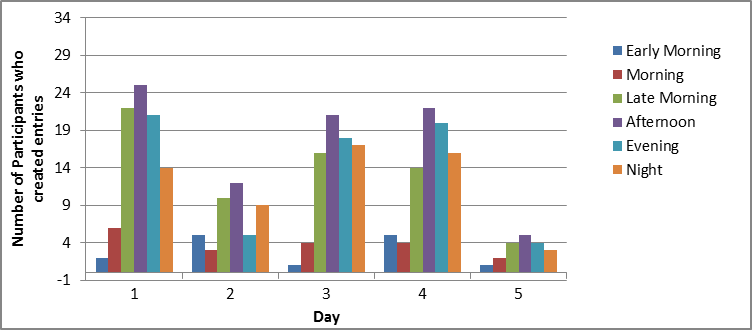
\includegraphics[ width =10cm ]{./images/cont1/chart14}}

\caption{Number of people who made entries over time}
\label{fig:chart14}

\end{center}
\end{figure}


Figure 14 shows how many participants created entries during each specified time period. With this population, it was fairly unpopular to make entries in the early morning (between midnight and 4am) and morning (4am-8am), while the late morning, afternoon and evening were the most popular times to make entries. 
\begin{figure}[ t ]
\begin{center}

\setlength\fboxsep{0pt}
\setlength\fboxrule{0.5pt}
\fbox{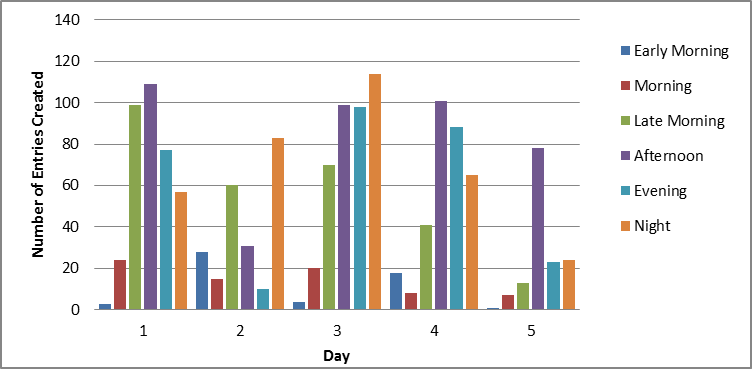
\includegraphics[ width =10cm ]{./images/cont1/chart15}}

\caption{Number of entries over time}
\label{fig:chart15}

\end{center}
\end{figure}

This chart shows a sum of all the entries entered during a particular time period each day. While the above chart showed the number of participants who made entries in that time period, this indicates how many entries those participants actually made. 

\textbf{What does this mean for the validation discrepancy?} Reviewing the charts, we see that day 1 has more people who made more entries earlier in the day, while on days 3 and 4 participants made entries primarily in the second half of the day, and created more entries in the second half of the day than in the first half of the day. This indicates that participants were probably entering their food closer to the time that they ate it on day 1, which means the day 1 entries probably more closely reflects what they actually ate. 

\subsubsection{Food Eaten Time}

\begin{figure}[ t ]
\begin{center}

\setlength\fboxsep{0pt}
\setlength\fboxrule{0.5pt}
\fbox{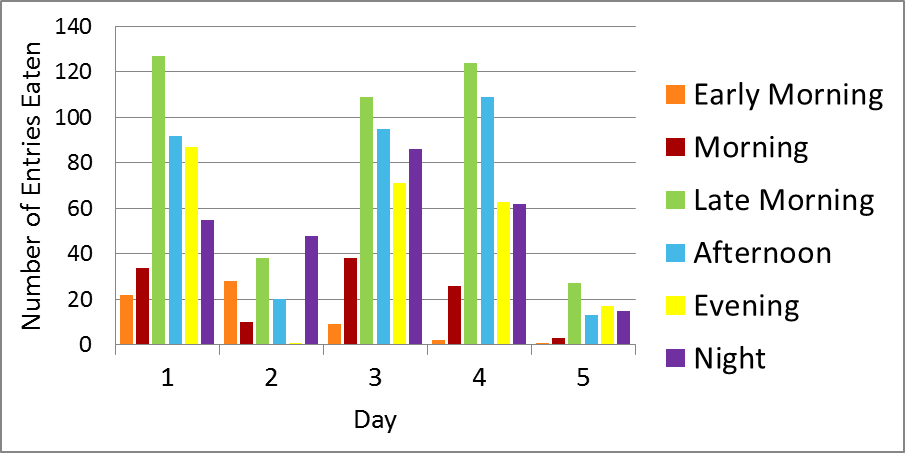
\includegraphics[ width =10cm ]{./images/cont1/chart16}}

\caption{Number of entries eaten over time}
\label{fig:chart16}

\end{center}
\end{figure}


This set of data consists of counting how many valid food diary entries were reported as being eaten in the given time period. The periods of time are again defined in 4-hour chunks, 6 periods per day, so 24 for the study time. 
For example, on Day 1, Late Morning, we see from the previous chart that ~100 entries were made, but we see in this chart that while only ~100 entries were made in this time period, about 120 foods were reported as eaten in this time period. 

A comparison of Figure 15 and Figure 16 indicates that participants likely made entries in the second half of the day capturing food that they ate in the first half of the day. 

\textbf{What does this mean for the validation discrepancy? }Similar to the entry creation time, usage on days 3 and 4 indicate patterns that correlate to greater error between what was eaten and what was entered. This appears less extreme on day 1, so again, the entries on day 1 probably more closely match what was actually eaten. 

\subsubsection{Entry Edits}

\begin{figure}[ t ]
\begin{center}

\setlength\fboxsep{0pt}
\setlength\fboxrule{0.5pt}
\fbox{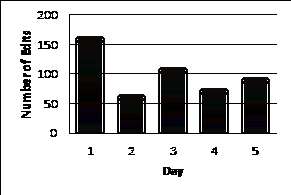
\includegraphics[ width =10cm ]{./images/cont1/chart17}}

\caption{Number of edits over time}
\label{fig:chart17}

\end{center}
\end{figure}


One indicator that users are becoming more familiar and comfortable with a piece of software or an interface is how many errors they make. In this study, the best indication we have for the number of errors people make throughout the whole study is how many edits they make.
 
The mean number of edits made by participants over the entire study is 13.559, with a standard deviation of 8.33. 

Figure 17 shows how many edits were made each day of the study, by all of the participants. The decrease in edits over time could indicate that participants were becoming more comfortable with the software, and making fewer errors in their entries. The increase on day 5 could reflect participants checking their entries to prepare for the completion of the study. 

\textbf{What does this mean for the validation discrepancy? }The high number of edits on day 1 could indicate that participants were being conscientious about ensuring that the records were correct. 

\subsubsection{Number Of Combos/Favorites And Their Use}
One of the features asked for many times in the focus groups the ability to save and use favorite foods, combinations, and recipes. In the validation study, 2 participants created 2 combos total, and used one of the combinations 2 times in their diary. 

\subsubsection{Combined For One Participant}
If this is at all helpful or interesting, I'll improve the chart. If not, I'll take it all out. 

To help put it in context, I show the graphs for two different participants. 
\begin{figure}[ t ]
\begin{center}

\setlength\fboxsep{0pt}
\setlength\fboxrule{0.5pt}
\fbox{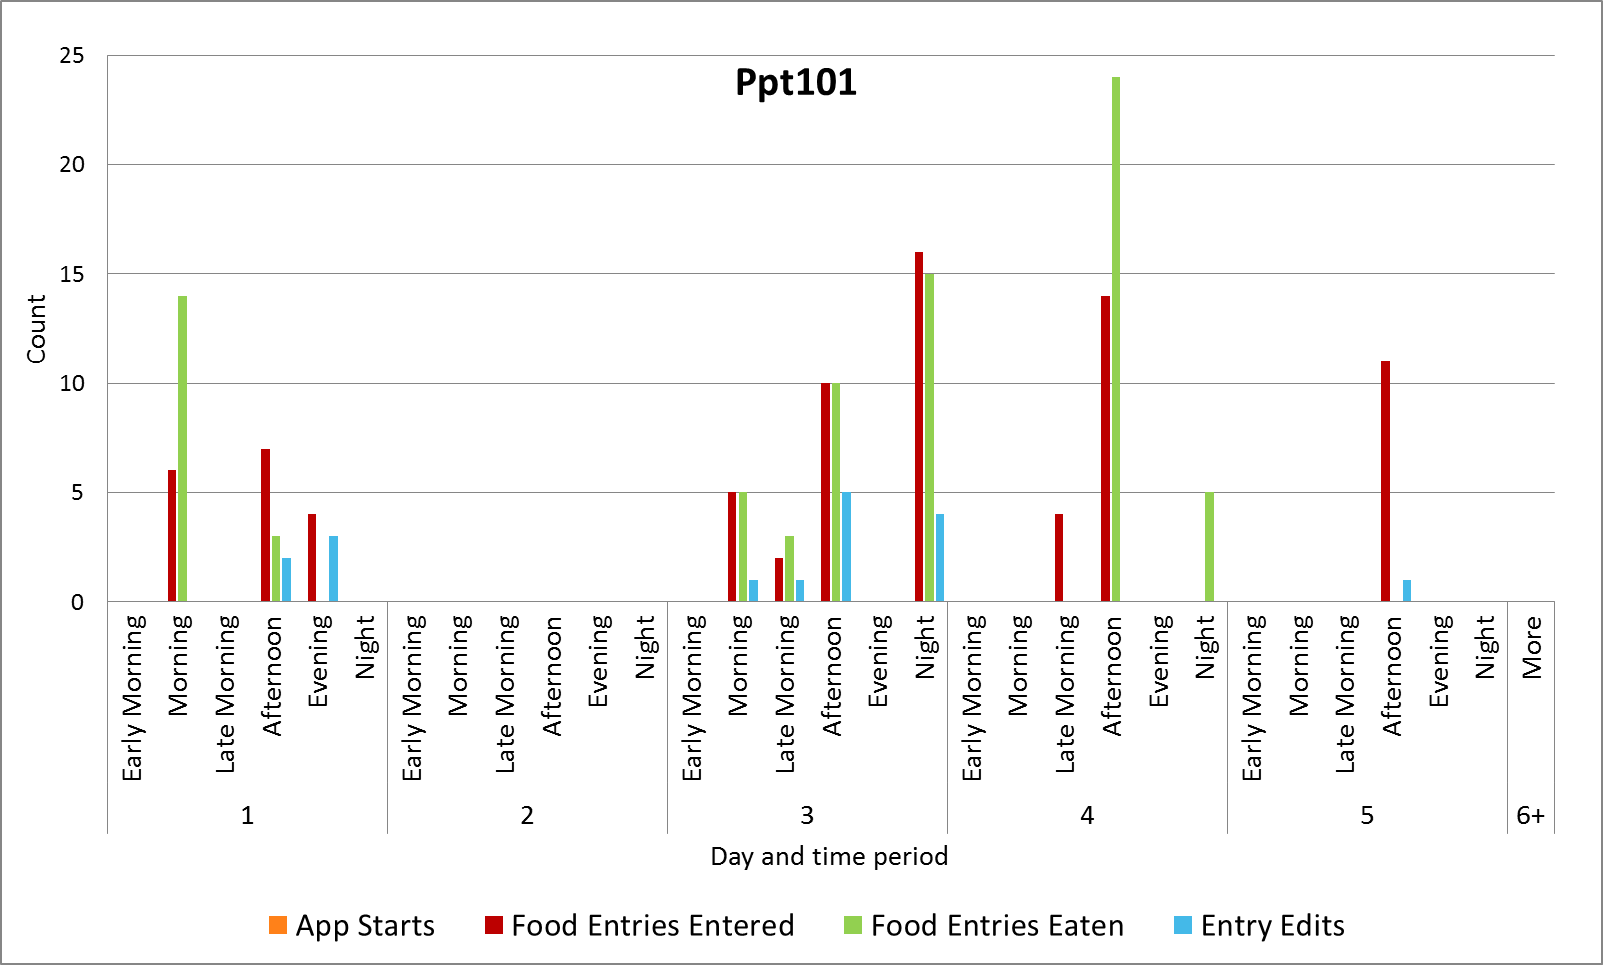
\includegraphics[ width =10cm ]{./images/cont1/chart18}}

\caption{Patterns of use, ppt101}
\label{fig:chart18}

\end{center}
\end{figure}

I start with Ppt101. As we see in this chart, there are App Starts (red). This is one of the participants who left the software running the entire time, which resulted in not being able to detect when the application was started. In addition to App Starts, this chart shows how many entries were entered in a given time period, as well as how many entries were reported as eaten in the given time period. Summed over all the days, the number of entries entered (green) equals the number of entries eaten (purple). On Day 1, in the morning, more foods were eaten than entered, but in the afternoon more foods were entered than eaten. This shows that the participant entered some of the food eaten in the morning, but later in the day went back and added some more entries. On Day 3, the participant was pretty consistent about entering entries when the food was eaten. On Day 4, many more entries were eaten in the afternoon and evening than were entered, and we can see that on Day 5, there were some more entries made, which explains that the participant went back and filled those entries in. 

\begin{figure}[ t ]
\begin{center}

\setlength\fboxsep{0pt}
\setlength\fboxrule{0.5pt}
\fbox{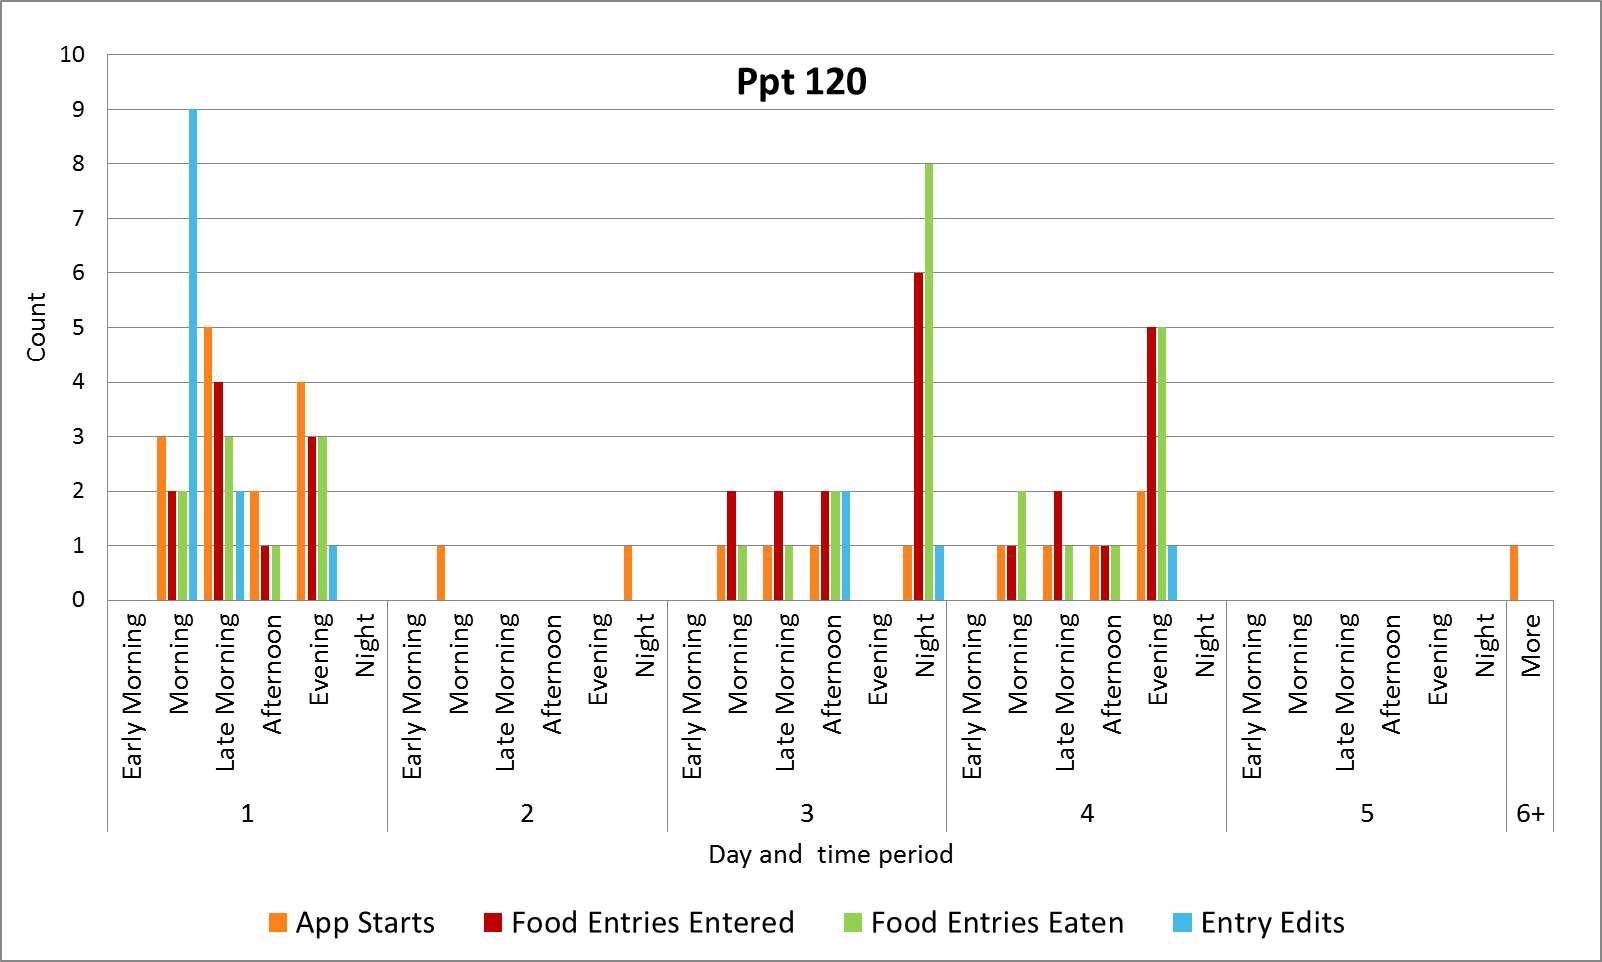
\includegraphics[ width =10cm ]{./images/cont1/chart19}}

\caption{Patterns of use, ppt120}
\label{fig:chart19}

\end{center}
\end{figure}

Ppt120 shows a more consistent interaction with the software. The app is started with each group of entries. For the most part, entries are entered at the time of eating, with a few edits. The first day generally shows more interaction with the software, which is consistent with a period of adjusting to it. Also, while there are many edits the first day, there are fewer edits in later days, which could indicate a greater familiarity with the software. 

\subsection{Discussion }
Previous research has identified factors that increase error in food diaries that people create. In the BALANCE validation study, we identified a discrepancy between what they entered and what was reported in a 24-hr recall. Previous work comparing food entries in an electronic food diary to a 24-hr recall found no significant difference [ref], but one difference between that study and this is that the 24-hr recall was performed a few days into a long-term study, rather than on the first day of a 3-day study. This raises the question of whether participants weren't as familiar with the software and device, and that the discrepancy may improve if the comparison was performed on the 3rd or 4th day. However, reviewing patterns of use as indicated by various metrics allowed us to understand that the first day of the study was probably the best data that would be collected in this study. 

\section{Overall Discussion}
The BALANCE project provides a rich dataset for us to begin understanding some of the challenges that people encounter when trying to self-monitor their food intake on mobile phones. Over all the studies, almost 50 people used the food diary for 3 days and provided detailed feedback. We were able to collect usage metrics on 34 of those participants, which helped us to better understand some of the patterns of use. All of this data also helped us to better understand how our metrics and methodology impacted the evaluation outcomes. I further elaborate on specific themes below. 

\textbf{Historical Context. }One thing that was a major issue for this project was the development and availability of mobile phones throughout the study period. The project began in 2008, and we were using state-of-the-art Nokia N80s. Soon, these were eclipsed by the N95s (with a larger screen and better tech specs). We began running the focus groups in spring 2009, finishing in the fall of 2009. The validation phase began in spring 2010, finishing in the fall (Sept?) of 2010. When we began the project, PDAs had been around for a while, but smartphones were just beginning to merge with PDAs by providing touch screens. Smartphones and appstores were very much a new thing-prior to this period, if someone bought a PDA or a smartphone and wanted to use any software that wasn't already pre-installed on the phone, they needed to be fairly tech savvy, purchase the software  and connect the phone to a computer to actually install it. Software usually required a stylus or joystick input, rather than the familiar touch, swipe or gesture interfaces that many are familiar with today. Today's appstores allow new software to be found and installed with just the touch of a finger. Altogether, this means that when we began this project, ``lay'' people (or maybe, less-technically-savvy) people hadn't really used their phone for much more than a basic phone, although they were increasingly aware of the notion of using ``apps'' on a phone. 

\textbf{Fast-changing Technology. }When we began the focus groups, the phone we gave to participants was considered very cool. One notable comment from a participant was that her teenage son thought she was so lucky to be able to use that phone. However, by the end of the project, comments from participants included things like ``the phone is so clunky and slow''. Indeed, one challenge we have going forward is that it's not likely to be the same phone model as the existing research that has been done. This is a challenge for researchers, because the process of an evolving interface and technology requires that hardware stay the same, or at least that the underlying technology doesn't change too drastically. However, for a ``research program'', it's important to be viewed by the participants as at least on par with currently available technology, if not cutting-edge. 

\textbf{Personal Devices. }When running studies using mobile phones, it's challenging to determine whether participants should carry a dedicated study-provided device (as well as whether the participant should use their own SIM in that device, or also carry their own personal device) or if the study software should be installed on a participant's personal device. As discussed in [ref Journal of HCI], the latter case may be preferable because the participants are familiar with the device, have all of their contact and other personal data on it, and therefore may be more likely to use the software on a regular basis. However, study prototypes may be unstable and cause the phone to crash, or otherwise interfere with the normal functioning of the phone. In the case of a study-provided device, the participant may be unfamiliar with the device, or have to carry two devices, which may make them less likely to use the software. 
In the BALANCE studies, we chose to provide study-owned devices to the participants to use in addition to their personal phones because of the technical requirements of the project. This could have impacted participant ability to adopt the software readily. 

\textbf{Consumer Savviness/Experience/Expectations.} One challenge of this research project is the difference between using a piece of software or a prototype as a research tool, or if the research is to inform the tool. One challenge of developing mobile applications is that the context matters. The way the software is used in situ can be very different than anticipated in the lab, and therefore an iterative approach is helpful for identifying those unanticipated []. On the other hand, when we are trying to improve on the design of the interface and services, we want feedback on it before building everything out. Therefore, the prototype that is being used to get user input on specific features might not be perfect. Users in the real world are less tolerant of imperfect or unrefined software. Even more, with mobile applications, it's difficult to recreate bugs that users find, and that makes it challenging to identify the true cause of a bug. Users are usually unable to provide enough information about the ``bug'' they report-as far as they are concerned, it just ``doesn't work'', or crashes. 

\textbf{Research Prototypes. }Given the concerns about consumer expectations of software, and that many mobile-phone food diaries already exist, why build a new one? Existing software is consumer-oriented, and a stand-alone product. This means we can't extend it to work with a novel visualization or the calorie-expenditure hardware, and it also means that we don't have access to the food diary data. Additionally, as discussed above, we are unable to instrument the software to inform us about how it is being used. 

\textbf{Database. }The food database had a huge impact on the overall design and implementation of the BALANCE software. There was a tension between needing a database that was big enough to have all the foods that many different people may encounter, but small enough to make it quick and easy to navigate. The information architecture of the database was important too-food groups and categories that are meaningful to experts and professionals may not be obvious to consumers. This is consistent with reports of the importance of high literacy abilities to navigate food and nutrition information [ref]. 

\textbf{Study Duration. }Choosing the duration of the final validation study required evaluating a tradeoff: reducing the duration put less burden on the participants, but they have less time to become familiar with the software and figure out how to make it fit into their daily schedules. Length of use also impacts the ability of the software to adapt to the participant. The personal database grows based on what people enter, making it easier to find and enter food, and the favorites features also provide a way to minimize interaction time. However, with a duration of three days, the time investment required for personalization will probably not have a large impact on the tracking process. 
While none of the evaluations showed that the BALANCE software enabled people to keep track of their food intake in a timely, complete and consistent manner throughout a day, this is consistent with other work that indicated technical malfunction prevented statistically significant results [ref]. Participants reported that the idea of tracking their food intake on their mobile phone was appealing, and offered valuable insight as to how we as designers and researchers may improve the process, particularly by reducing the amount of effort that goes in to the food intake capture. This allows us to raise the question of whether people will be able to enter food intake on a consistent basis if we reduce the amount of effort, in terms of time, physical entry (entering text or pushing buttons) and mental activity (how much the user needs to think about the process). This is addressed in the next chapter. 

\section{Summary}
In this chapter, I describe the BALANCE project, focusing primarily on the design and development of the food diary component of the project. I also provide an HCI-oriented evaluation of the use of the BALANCE software by participants in-situ, to better understand the results of the more quantitative, [medical]-oriented evaluation. This HCI-oriented evaluation identified that one important barrier to participants creating complete, comprehensive and timely food entries is due to the database. I document the challenges of using a food database on resource-constrained devices such as mobile phones, and [prove that nothing more could be done to improve the database experience with this technology]. The database is challenging to navigate and requires mental effort, particularly in real-world context, in addition to requiring time-consuming text entry. User feedback indicated that people understand the value that dietary self-monitoring could provide, but that the BALANCE food diary required too much time. It also indicated that people might be willing to accept a less detailed accounting of their food intake in exchange for a less challenging/time-intensive collection process. 

 
